\documentclass{beamer}
\usepackage{float}
\usepackage{multicol}
\usepackage{bm}
\usepackage{amsmath,amsthm,amsfonts,amssymb,amscd, fancyhdr, color, comment, graphicx, environ}

%Information to be included in the title page:
\title{Diffusion-based Vocoding for Real-Time Text-To-Speech}
\author{Lukas Gardberg}
\institute{LTH}
\date{\today}

\begin{document}

\frame{\titlepage}

\begin{frame}
\frametitle{Presentation Layout}
\begin{itemize}
    \item Problem Introduction
    \item Past Work
    \item Problem Statement / Goals
    \item Quick background
    \item TODO: Add more
\end{itemize}
\end{frame}

% ---------- %

\begin{frame}
\frametitle{Typical TTS Pipeline}

\vspace{1cm}

\begin{center}
{\large
    Text \quad $\longrightarrow$ \quad Speech
}
\end{center}

\vspace{1cm}

\begin{figure}[H]
    \centering
    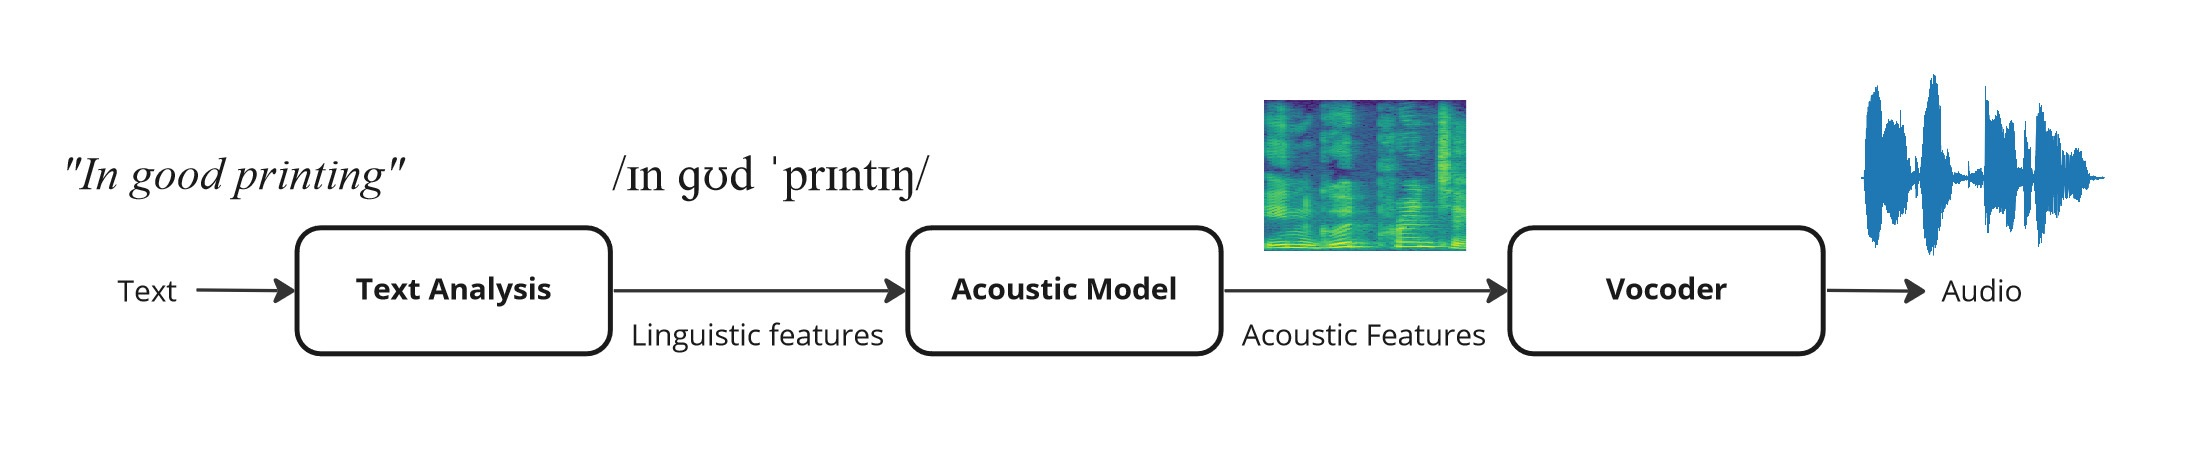
\includegraphics[width=1\textwidth]{images/TTS.jpg}
\end{figure}

\vspace{1cm}

\begin{multicols}{3}
    \begin{center}

    Text Analysis

    \vfill\null
    \columnbreak

    Acoustic Model

    \vfill\null
    \columnbreak

    Vocoder

    \end{center}
\end{multicols}

\end{frame}

% ---------- %

\begin{frame}
    \frametitle{The Phase Reconstruction Problem}

    \begin{itemize}
        \item Goal: Reconstruct signal $\bm{x}$ from its mel spectrogram $\bm{S}_{\text{mel}}$
    \end{itemize}
    
    \pause

    \begin{figure}[H]
        \centering
        \includegraphics[width=1\textwidth]{images/Phase_reconstruction.png}
    \end{figure}
    
\end{frame}

% ---------- %

\begin{frame}
    \frametitle{The Phase Reconstruction Problem}

    How has this been done before?

    \vspace{1cm}

    \begin{itemize}
        \pause
        \item Griffin-Lim Reconstruction
        \pause
        \item Autoregressive Neural Networks (WaveNet)
        \pause
        \item GANs (HiFi-GAN)
        \pause
        \item Diffusion (DiffWave)
        \pause
        \item ...and more
    \end{itemize}
    
    
\end{frame}

% ---------- %

\begin{frame}{Diffusion}
\large
    \begin{itemize}
        \setlength\itemsep{1.5em}
        \item Main idea 
        \item Where do Neural Networks come in? 
        \item How can it be used for vocoding?
    \end{itemize}

\end{frame}    

% ---------- %

\begin{frame}{Diffusion}

Collected training data $\mathbb{X} = \{ \bm{x}^{(i)} \}_{i=1}^N$ drawn as $\bm{x} \sim q_{\text{data}}$.

\vspace{0.5cm}
\pause
Want to be able to generate \textit{new data} from the "target" distribution!

\vspace{0.5cm}
\pause
How?

\end{frame}

% ---------- %

\begin{frame}{Diffusion}

    \begin{itemize}
        \setlength\itemsep{1.5em}
        \item Transform data from a simple distribution $p_{\text{latent}}$ (e.g. noise) into the complex target distribution $q_{\text{data}}$
        \pause
        \item In one step is hard, in several steps easier
        \pause
        \item Also easy to \textit{destroy} data into noise, hard to do the inverse
        \pause
        \item Teach a model to perform each "denoising" step
    \end{itemize}

\end{frame}

% ---------- %

\begin{frame}{Forward Process}

$T$: Number of diffusion steps \\
\pause
$\bm{x}_0$: Ground truth sample \\
\pause
$\bm{x}_t$: Sample after $t$ diffusion steps \\
\pause
$\bm{x}_T$: Final sample, hopefully close to $p_{\text{latent}}$ \\

\vspace{0.6cm}

\pause

\begin{align*}
\bm{x}_t \sim & \, q(\bm{x}_t \mid \bm{x}_{t-1}) = \, \mathcal{N}(\bm{x}_t \, ; \, \sqrt{1 - \beta_t} \bm{x}_{t-1}, \beta_t \bm{I}) \\
\bm{x}_t = & \, \sqrt{1 - \beta_t} \bm{x}_{t-1} + \beta_t \bm{\varepsilon}, \quad \bm{\varepsilon} \sim \mathcal{N}(\bm{0}, \bm{I}) \\
\end{align*}

\vspace{0.6cm}

\pause

Variance schedule $\beta_t \in [0, 1]$: At which "rate" we tend towards a unit Gaussian

\end{frame}

% ---------- %

\begin{frame}{Forward Process}
    Quick way to get a noisy sample $\bm{x}_t$:

    \vspace{0.6cm}

    \begin{align*}
        \bar{\alpha}_t = & \, \prod_{i=1}^t (1 - \beta_i) \\
        \bm{x}_t \sim & \ q(\bm{x}_t \mid \bm{x}_{0}) = \mathcal{N}(\bm{x}_t \, ; \, \sqrt{\bar{\alpha}_t} \bm{x}_0, \sqrt{1-\bar{\alpha}_t} \bm{I}), \\
        \bm{x}_t = & \, \sqrt{\bar{\alpha}_t} \bm{x}_0 + \sqrt{1-\bar{\alpha}_t} \bm{\varepsilon}, \quad \bm{\varepsilon} \sim \mathcal{N}(\bm{0}, \bm{I}) \\
    \end{align*}
    
\end{frame}

% ---------- %

\begin{frame}{Forward Process}

    \begin{figure}[H]
        \centering
        \includegraphics[width=0.79\textwidth]{images/density2.png}
    \end{figure}

\end{frame}

% ---------- %

\begin{frame}{Backward Process}

\begin{itemize}
    \setlength\itemsep{1.5em}
    \item We want to be able to generate samples using the backward process
    \pause
    \item Model each transition as $p_{\theta}(\bm{x}_{t-1} \mid \bm{x_t}) = \mathcal{N}(\bm{x}_{t-1} \, ; \, \bm{\mu}_{\theta}(\bm{x}_t, t), \bm{\Sigma}_{\theta}(\bm{x}_t, t))$
\end{itemize}
    
\end{frame}

% ---------- %

\begin{frame}{Backward Process}

    \begin{figure}[H]
        \centering
        \includegraphics[width=0.79\textwidth]{images/density.png}
    \end{figure}

\end{frame}

% ---------- %

\end{document}